\documentclass[a4paper,12pt,titlepage]{article}
\usepackage[polish,english]{babel}
\usepackage[utf8]{inputenc}
\usepackage[T1]{fontenc}
\usepackage{tabularx}
\usepackage[pdftex]{graphicx}
\usepackage{amsmath}
\usepackage{geometry}
\geometry{lmargin=3cm,rmargin=3cm,tmargin=3cm,bmargin=3cm}
\title{Physics of The Critical Point\\\small Summation of co-op part of project}

\author{Kamil Kaczmarczyk \\ Mariusz Jędraczka}
\begin{document}
  \maketitle
  \section{Introduction}
  As our project evolved we were given few interesting tasks to deal with. Since first step of our whole group was 1D Ising Model thus
  we begun with examining energy of lattice, its correlation function as well as specific heat function. We were also given a task to 
  observe evolution of the system and to test its behavior in matter of clusters distribution.
  \section{Energy function and mean energy correlation function}
  Energy of whole lattice is defined, through direct solution of the model, by following equation of hamiltonian
  \begin{equation}
    H=-J\sum_{i,j:|i-j|=1}^{N}{s_is_j}
  \end{equation}
 
  And thus mean energy value per spin in $N$ - spin chain is given by
  \begin{equation}
    E=\frac{H}{N}
  \end{equation}

  In our model $J=1$ which simplifies expression.
  
  As it can be seen our model considered only summing over nearest neighbours with periodic boundary conditions - first and the last element
  of the spin chain were connected.
  
  What are our expectations of the energy behavior as we change temperature of the system? As the temperature rises the energy per spin
  should also be rising. The orientation and the distribution of the spins is also connected with this - in high temperature we expect our system
  to be in disordered state while with lowering the temperature spins tend to form clusters - objects consisting of paralell oriented spins.
  Should the whole lattice be oriented in one direction the energy per spin ought to be unit.
  
  Since 1D Ising model has analytic solution thus we can compare our results with exact formula.
  \begin{equation}
    E_{theo}=-tanh\left(\frac{1}{T}\right)
  \end{equation}
  On the next page we have placed adequate plot that shows what we were able to observe and calculate.
  \newpage
  \begin{figure}[h]
    \centering
    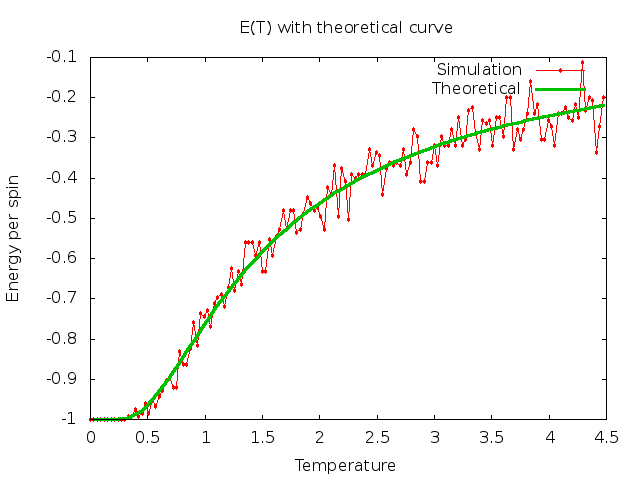
\includegraphics[scale=0.5]{plots/IsingTestE1D_teo.png}
  \end{figure}
  As one can see on the plot above - theoretical curve is covering quite well points taken with Monte Carlo methods. Theory is in good
  agreement with calculations as well as our predictions for the lattice - if we'd let temperature rise to infinity spins would be in
  total disordered state - half of them would be oriented up and half down. In this case energy of whole system would be zero and this
  is what we observe in both: $-tanh\left(\frac{1}{T}\right)$ function and the behavior of calculated points, in limit they go to $0$.
 
  What concerns the algorythm is that this results were easy to obtain since energy was simple sum over all pairs of neighboring spins (equation $1$)
  with periodic boundary conditions: last and the first spin were connected. After dividing this sum by number of all spins one can get energy of the
  system per spin.
 
  What we were interested next was the matter of energy correlation between spins in the chain. Correlation function that we used in 
  algorithms was following:
  \begin{equation}
    G_E(x)=\left<E\left(x_0\right)E(x)\right>-\left<E\right>^2
  \end{equation}
  where $\left<E\right>^2$ is the energy of whole system per spin, and the first term is the multiplication of energy of two spins that
  are at distance of $x$. Since $G_E$ is function of distance we check what is its value from formula above for every spin with energy $E_0$
  and at distance $x\ \epsilon \left[1;max\right]$. Where $max$ parameter is simply maximum distance on which we want to check the 
  correlation function. Every spin gives us $max-1$ correlation function. If we measure value of this function for every spin putting 
  its energy for $E_0$ and add considering the same distance we can then get mean value by dividing each element in table of correlations
  (or vector, it's only the matter of names) by number $N$ - size of the lattice. 
  
  Anticipating some questions - by computing correlation values for different spins we are increasing the distance only in one direction
  so when we swtich for next spin and measure correlation for it we will never go back, and each pair of spins is always taken only once.
  
  \newpage
  Let this be some introduction, now look at Monte Carlo results shown on the plot below. To clarify - it is not a single measurement of
  a static spin chain. For different temperatures we've taken 1 hundred measurements to obtain some decent statistic. We let our system
  to evolve at fixed temperature and than averaged the results over $100$.
  \begin{figure}[h]
    \centering
    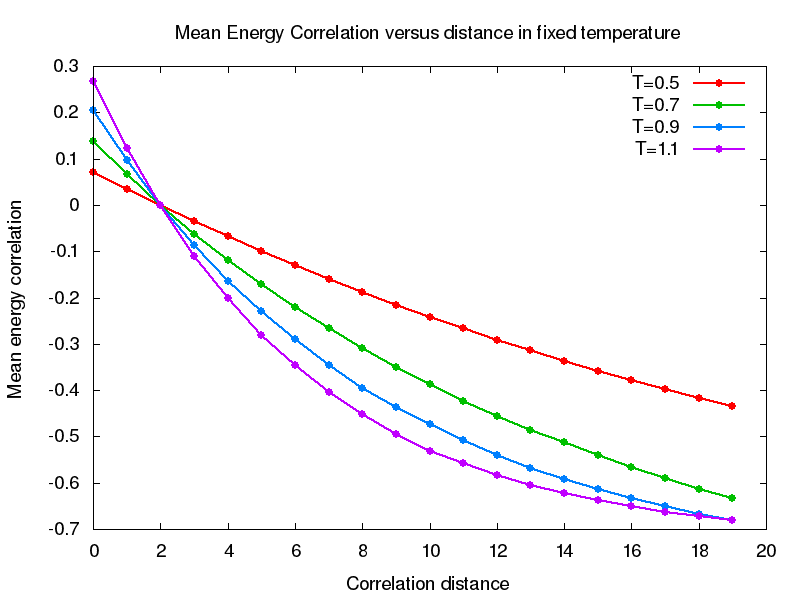
\includegraphics[scale=0.5]{plots/IsingTestMeanECorrelation_T.png}
  \end{figure}
  
  One can clearly see that as the temperature grows mean energy correlation distribution flattens.
  
  \begin{verbatim}
    Additional comment needed
  \end{verbatim}

  
  
\end{document}
